\documentclass[10pt]{article}
\usepackage[polish]{babel}
\usepackage[utf8]{inputenc}
\usepackage[T1]{fontenc}
\usepackage{amsmath}
\usepackage{amsfonts}
\usepackage{amssymb}
\usepackage[version=4]{mhchem}
\usepackage{stmaryrd}
\usepackage{graphicx}
\usepackage[export]{adjustbox}
\graphicspath{ {./images/} }

\begin{document}
\begin{enumerate}
  \item Na ile sposobów można dojść z punktu \((0,0)\) do punktu o współrzędnych \((n, k)\), gdzie \(n\) i \(k\) są liczbami naturalnymi, jeżeli możemy wykonywać jedynie kroki o jeden w prawo lub o jeden do góry. Odpowiedź uzasadnij.
  \item Ile jest ciągów ( \(a, b, c, d\) ) liczb całkowitych nieujemnych spełniających równanie:
\end{enumerate}

\[
a+b+c+d=21
\]

\begin{enumerate}
  \setcounter{enumi}{2}
  \item Trzy prostokąty o wymiarach \(1 \times 2\) są położone jak na rysunku obok (punkty A, B, E, F są współliniowe). Jakie jest pole trójkąta HKL?\\
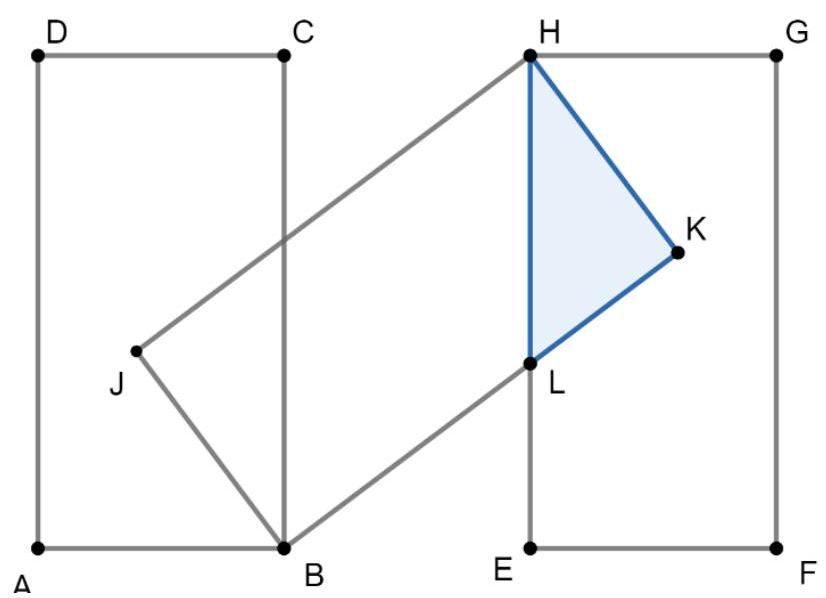
\includegraphics[max width=\textwidth, center]{2024_11_21_59abd5fb4069b0a9805eg-1}
\end{enumerate}

\end{document}